%!TEX root = ../../super_main.tex

\section{Customer Interaction}
\label{sec:customer_interaction}

To provide customers with a way of defining campaigns, and retrieving information from the system, a website have been created. Interacting with this website is only be available to customers, who may interact with the system in two ways, depending on their intent.  Customers can, through a Graphical User Interface (GUI), browse their previously created campaigns along with creating new ones. Alternatively, if customers wish to retrieve the gathered labeled training data, they may utilize an Application Programming Interface (API). Both ways of interacting with the system will be described in this section.
\\\\
When visiting this site, customers a presented with the page seen in \figref{fig:web_welcome}. Everybody, meaning both customers, participants, and people outside these categories, have access to this page, meaning that this welcome-page could be utilized to give the visitors more information regarding the system and the possibilities there lies within, which might lead to them becoming either customers or participants. 

\todo[inline]{Skriv at web-delen er et ekspertsystem og konsekvenserne af dette}

\todo[inline]{MÅSKE: Indsæt de mockups vi har lavet af web-delen}

\todo[inline]{skriv at screenshot er lavet på dev, men hvis folk vil ind og se den bedste side evar skal de ind på prod}
 

\todo[inline]{Skriv at URLen i alle screenshots er ``forkert'', og skriv at hvis folk vil besøge den, og oprette campaigns osv, så er den tilgængelig på www.x.dk/data}

\todo[inline]{Beskriv \tabref{tab:browser_routes} i introduktionen }

\begin{table}[!htbp]
    \centering
    \begin{tabular}{|l|l|} 
        \hline
        \textbf{Type} & \textbf{URL}                            \\ \hline 
        \mono{GET}    & \mono{campaigns}                        \\ \hline 
        \mono{POST}   & \mono{campaigns}                        \\ \hline 
        \mono{GET}    & \mono{campaigns/create}                 \\ \hline 
        \mono{GET}    & \mono{campaigns/\{campaign\}}           \\ \hline 
        \mono{GET}    & \mono{campaigns/\{campaign\}/snapshots} \\ \hline 
        \mono{GET}    & \mono{home}                             \\ \hline 
        \mono{POST}   & \mono{login}                            \\ \hline 
        \mono{GET}    & \mono{login}                            \\ \hline 
        \mono{GET}    & \mono{logout}                           \\ \hline 
        \mono{POST}   & \mono{password/email}                   \\ \hline 
        \mono{POST}   & \mono{password/reset}                   \\ \hline 
        \mono{GET}    & \mono{password/reset/\{token?\}}        \\ \hline 
        \mono{POST}   & \mono{register}                         \\ \hline 
        \mono{GET}    & \mono{register}                         \\ \hline 
    \end{tabular}
    \caption{The routes that the is used on the website.}
    \label{tab:browser_routes}
\end{table}

% Welcome not logged in
\begin{figure}[!htbp]
\centering
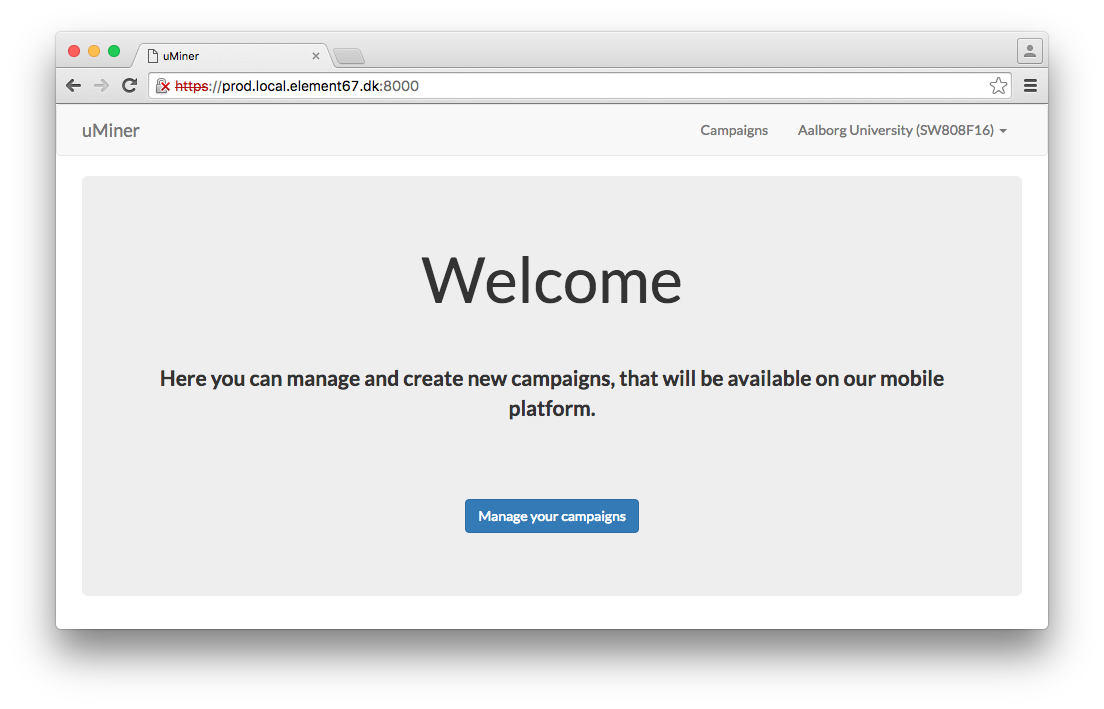
\includegraphics[width=\linewidth]{user_interfaces/web/web_welcome}
\caption{Welcome page.}
\label{fig:web_welcome}
\end{figure}
\FloatBarrier

\subsection{Registration and Logging In}

To gain access to the features of the website, customers must first log in. If the customer does not have a login, one can be created through the register page, as seen in \figref{fig:web_register}. The \emph{name} input field will later be used to show participants who created the different campaigns. Please note that the same name can be shared by multiple accounts. This means that multiple accounts can be associated with \emph{Aalborg University}, for instance. Currently, everybody can register an account, but one could imagine that some level of verification might be required, so people cannot impersonate companies or persona. When the customer is registered, he/she can log in through the login-page seen in \figref{fig:web_login}.  

% Register
\begin{figure}[!htbp]
\centering
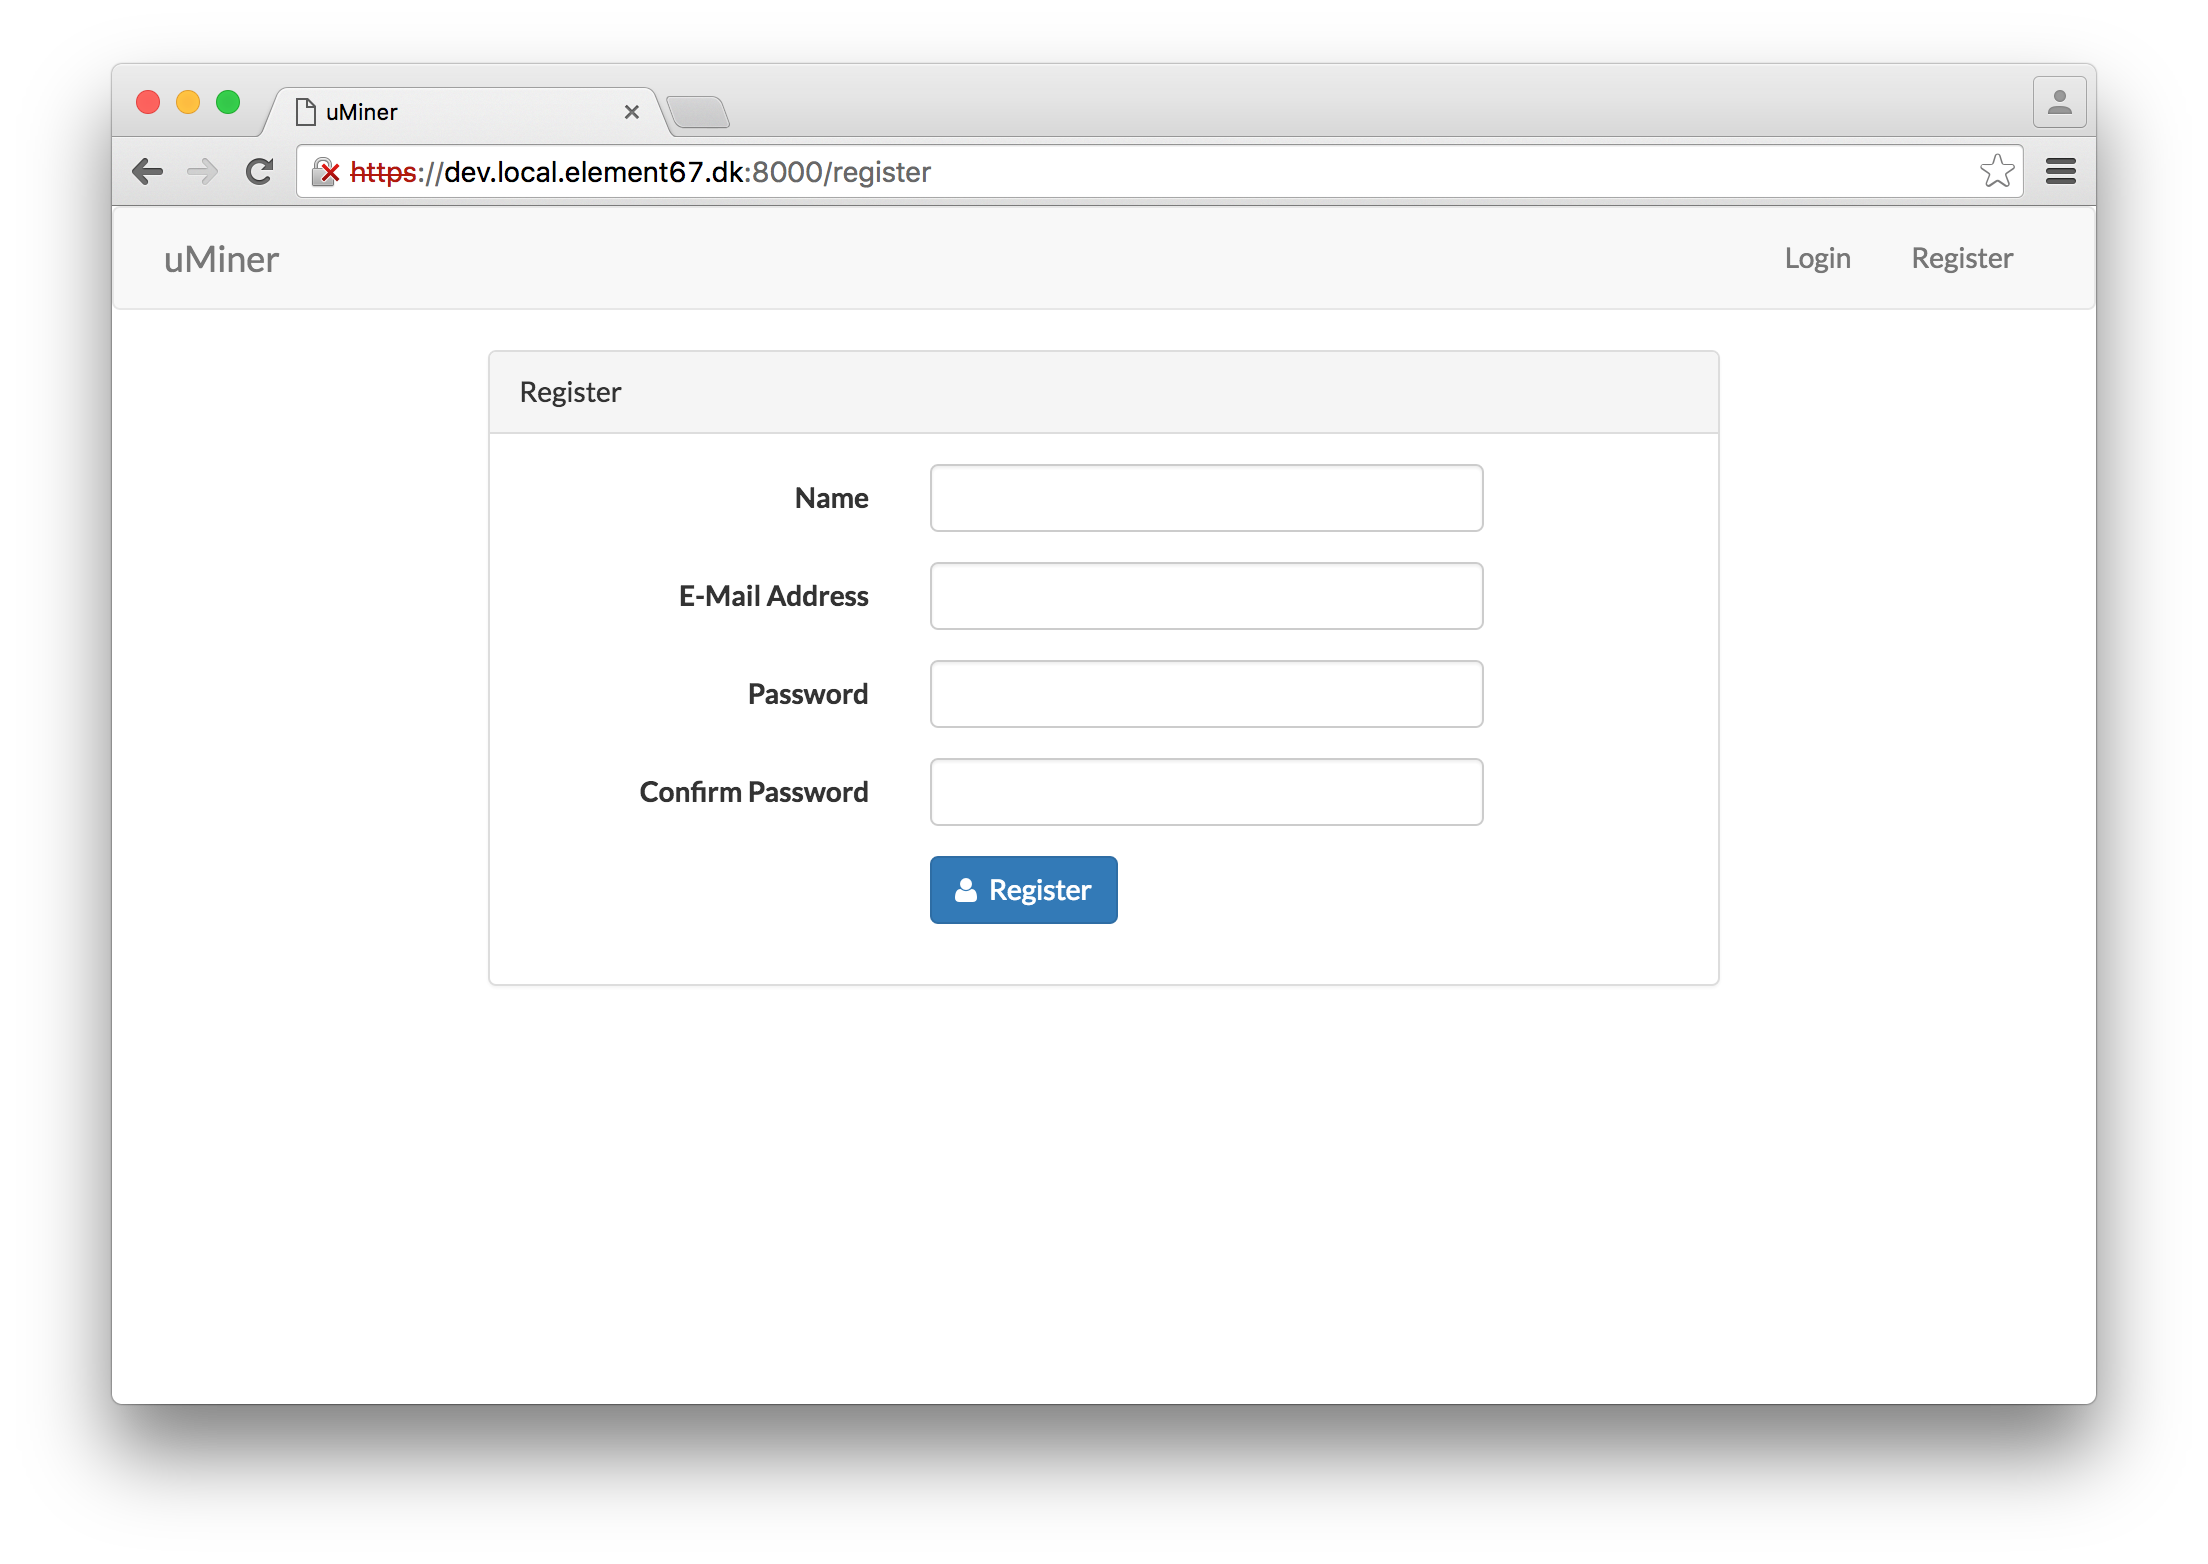
\includegraphics[width=\linewidth]{user_interfaces/web/web_register}
\caption{Register page.}
\label{fig:web_register}
\end{figure}
\FloatBarrier

% Login
\begin{figure}[!htbp]
\centering
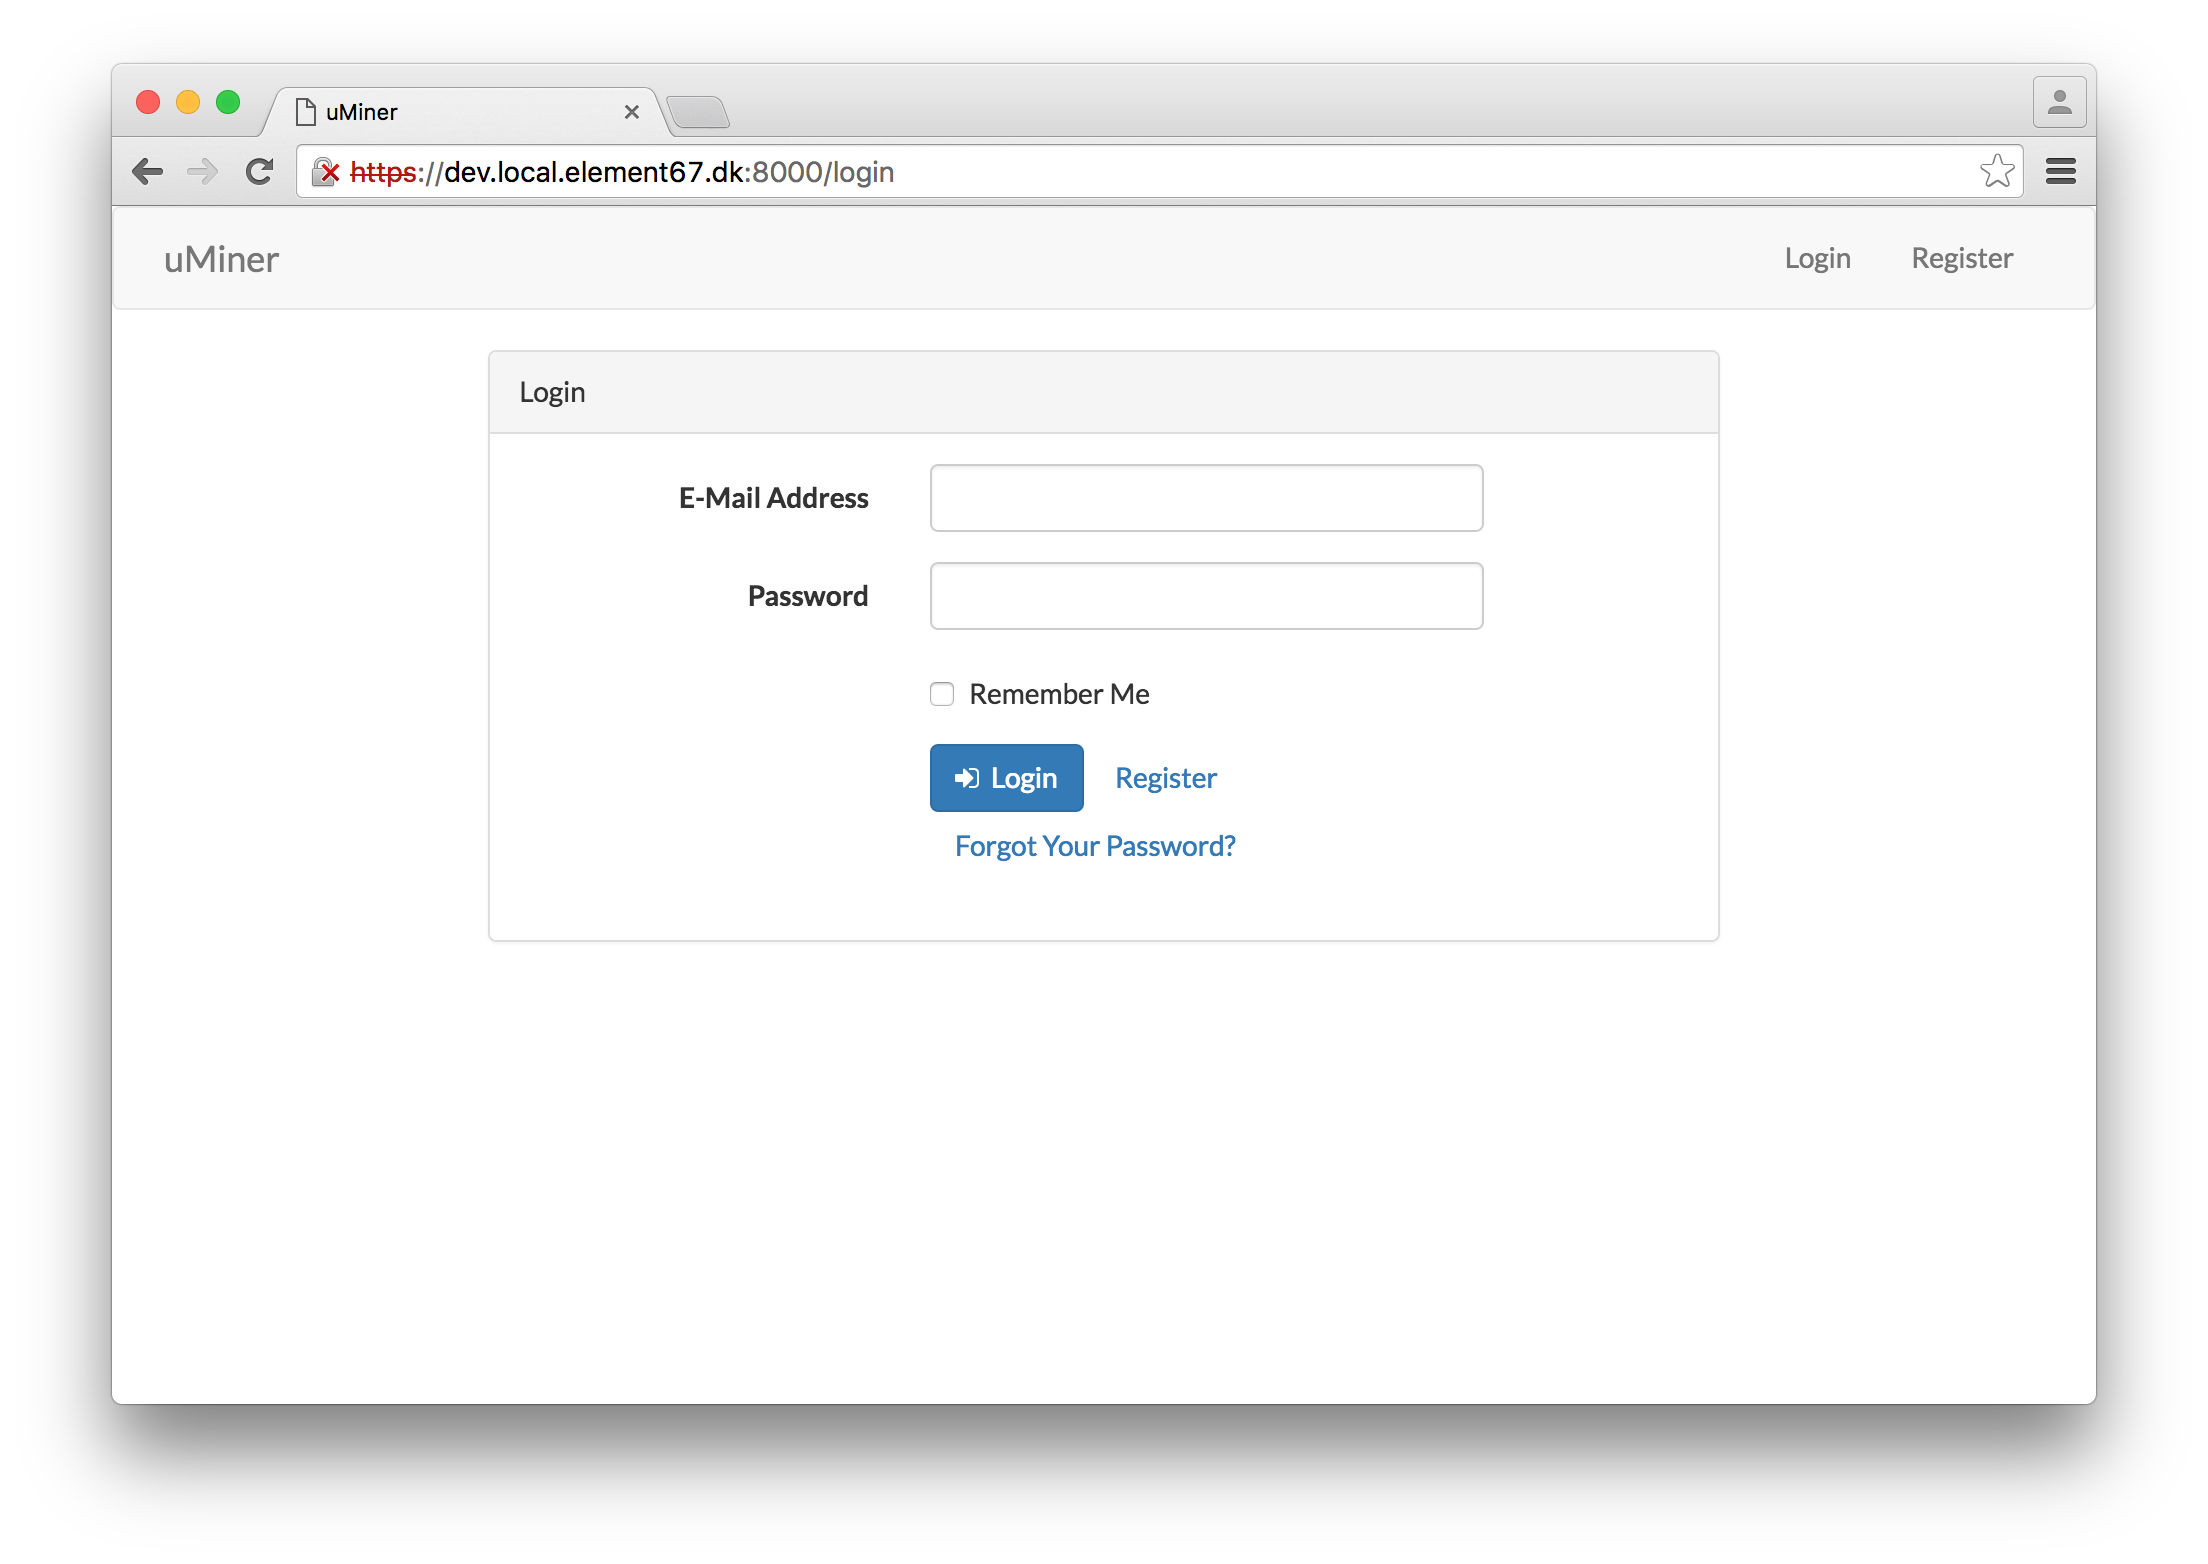
\includegraphics[width=\linewidth]{user_interfaces/web/web_login}
\caption{Log in page.}
\label{fig:web_login}
\end{figure}
\FloatBarrier

\subsection{Creating Campaign}

When logged in, customers can now create campaigns. This is done through the site seen in \figref{fig:web_create_campaign}. Here, customers will have to specify different details regarding the campaign. To give customers an ideas of how the participants will view this information, a mobile phone is included on the page, showing the mobile application. Please note that this is only an indication of how it will look, since different phones, with different screen sizes, font settings, etc. will influence the look of the application. A detailed description of all the input fields that the customer will have to fill out is described below.

\begin{description}
    \item[Campaign title] is used to give participants a rough idea of what the campaign will be used for. This information will visible when participants are browsing campaigns (\figref{fig:public_campaigns}) and when viewing details regarding the campaign (\figref{fig:campaign_specification}).

    \item[Campaign description] will provide participants with a detailed description of the campaign. This text could possibly contain motivational factory, inclining participants to participate in that specific campaign. This information is only available to participants when viewing the specifications of the campaign (\figref{fig:campaign_specification}).

    \item[Campaign author] cannot be specified directly by the customer, but is instead depending on the name of the account that the participant is logged into. Like the campaign title, this information will be included when participants are browsing campaigns (\figref{fig:public_campaigns}) and when viewing details regarding the campaign (\figref{fig:campaign_specification}).

    \item[Campaign availability] can be specified through the checkbox directly below the description input field. This checkbox is marked by default, making the campaign public available (i.e making it visible for participants browsing campaigns through the view seen in \figref{fig:public_campaigns}). Unchecking this checkbox will cause the campaign to be private, effectively meaning that customers will have to distribute the campaign identifier in order to get participants.

    \item[Sensors] is a section which allows customers to specify which sensors they would like to gather information from. Sensors are divided into four categories, roughly describing the information that the sensors will collect. In the current implementation of the system, all of these sensors are marked as ``nice to have'', effectively meaning that participants can subscribe to the campaign regardless of the sensors in their phone. Customers might be interested in excluding participants who does not have some essential sensors \todo{Det er en ret stor del af vores projekt - vi burde måske skrive noget mere om vores overvejelser mht. sensore der kan komme og gå, som eksempelvis smart watches etc.}. 

    \item[Sample and measurement] consists of five different input fields. The \emph{Snapshots per Campaign} input is used to specify how many snapshots the participant must collect before completing a campaign. However, in the current implementation of system, this property is not used, meaning that participants will continue to contribute until unsubscribing from the campaign. The \emph{Measurement per Sample}- and \emph{Measurement delay} input fields will change the length of a sample; while the \emph{Samples per Snapshot}- and \emph{Sample delay} input fields will change the length of a Snapshot. Please note that this way of specifying snapshots differs from the internal structure, explained in \todo{ref}. We did this, since customers might find it easier to specify the delay between measurements and samples, rather than having to calculate the different frequencies. The concept of delay, amount of measurements, samples etc. might still be difficult to grasp, so we have included a illustration of a time-line. This could possibly aid customers in specifying the different parameters. Ideally, the figure should be responsive, and automatically update whenever customers change the input fields \todo{Please halp. Det er svært at forklare og endnuværre at forstå!}. 

    \item[Questionnaire placement] will indicate when participants are prompted with questions. As described previously, in \secref{sub:answering_questionnaired}, this can either be in the beginning, or the end of a snapshot. We have also had some considerations in regards to when participants should be prompted, which are also described in \secref{sub:answering_questionnaired}.

    \item[Questionnaire] specification simply consists of a sequence of questions. Questions can be re-arranged by dragging them up or down in the list. When answering questions, the participants will receive the questions in the same order, as they are presented on this page. Please note that if the customer does not specify any questions, participants will never be prompted to fill out a questionnaire regarding that campaign. 
\end{description}

% Create campaign
\begin{figure}[!htbp]
\centering
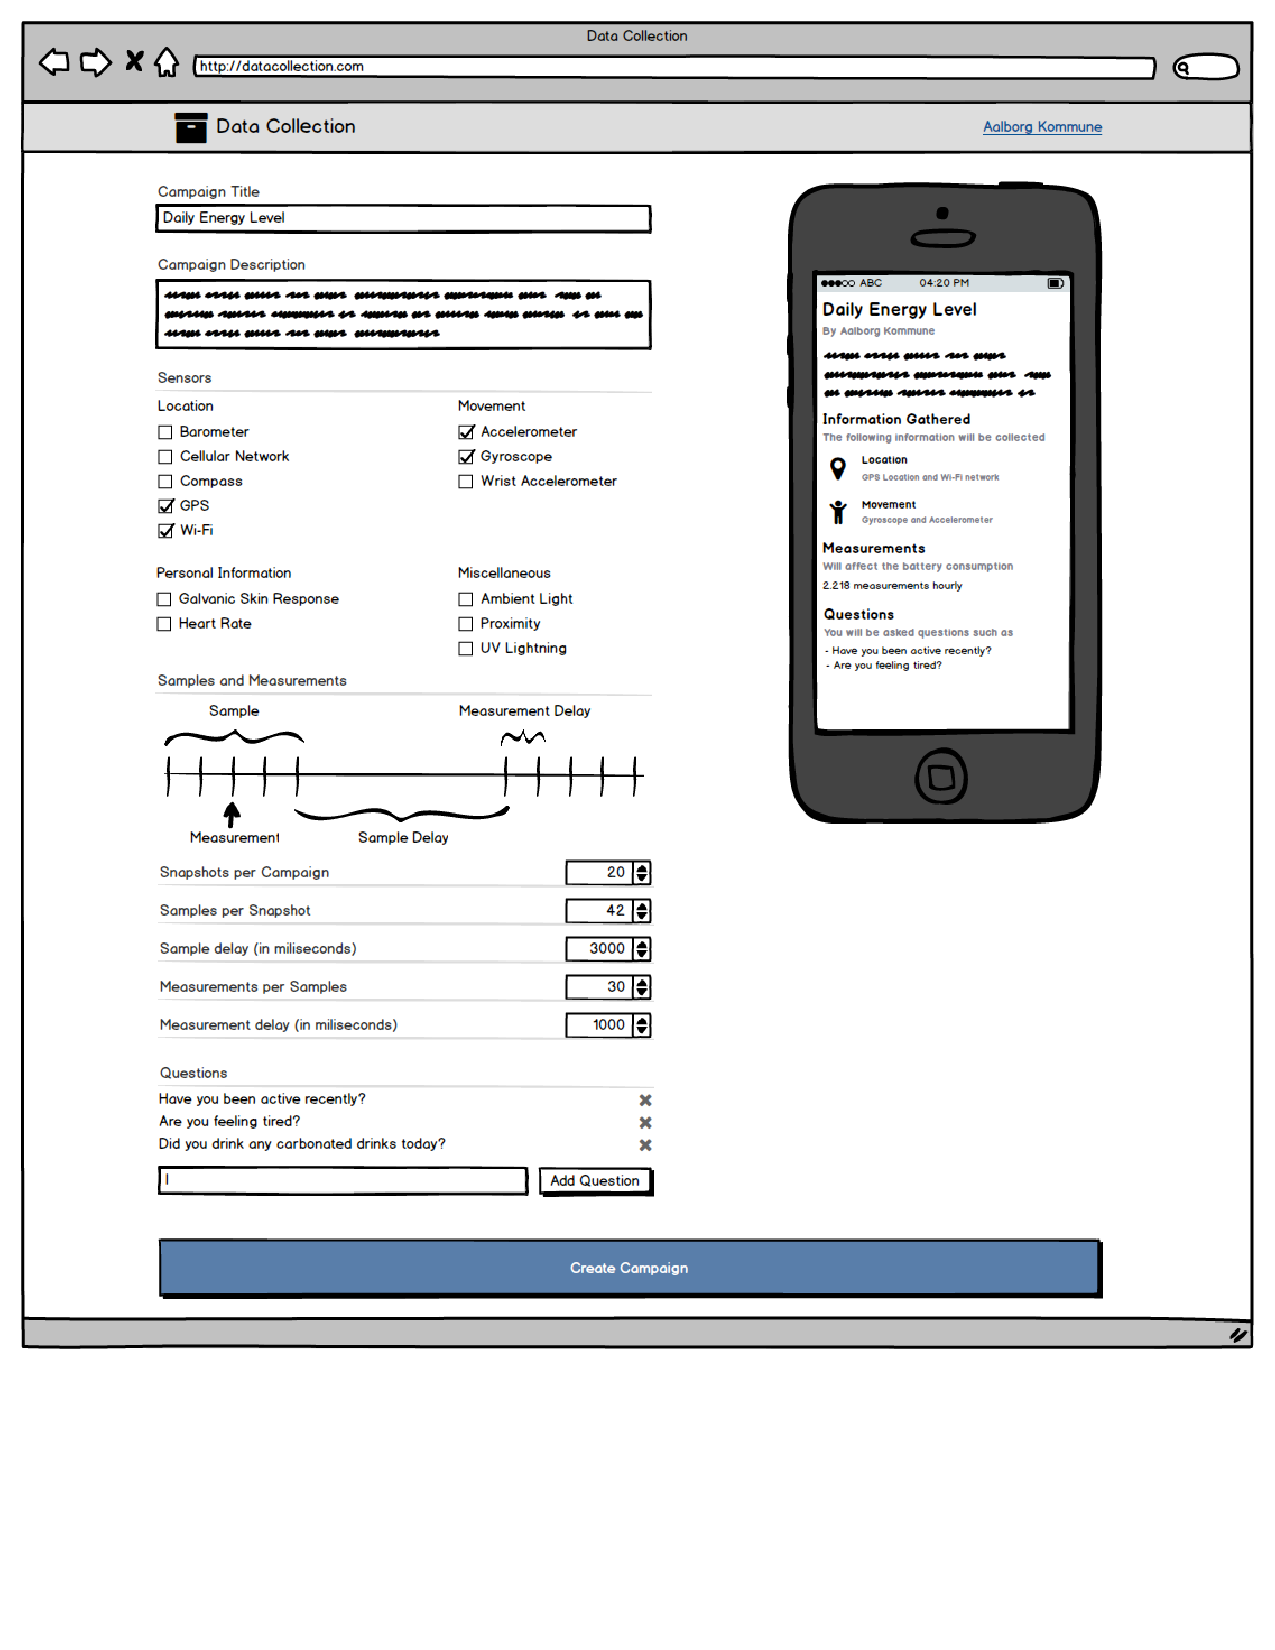
\includegraphics[width=\linewidth]{user_interfaces/web/web_create_campaign}
\caption{Creating Campaigns.}
\label{fig:web_create_campaign}
\end{figure}
\FloatBarrier

\subsection{Viewing Campaign Details}

% View campaign
\begin{figure}[!htbp]
\centering
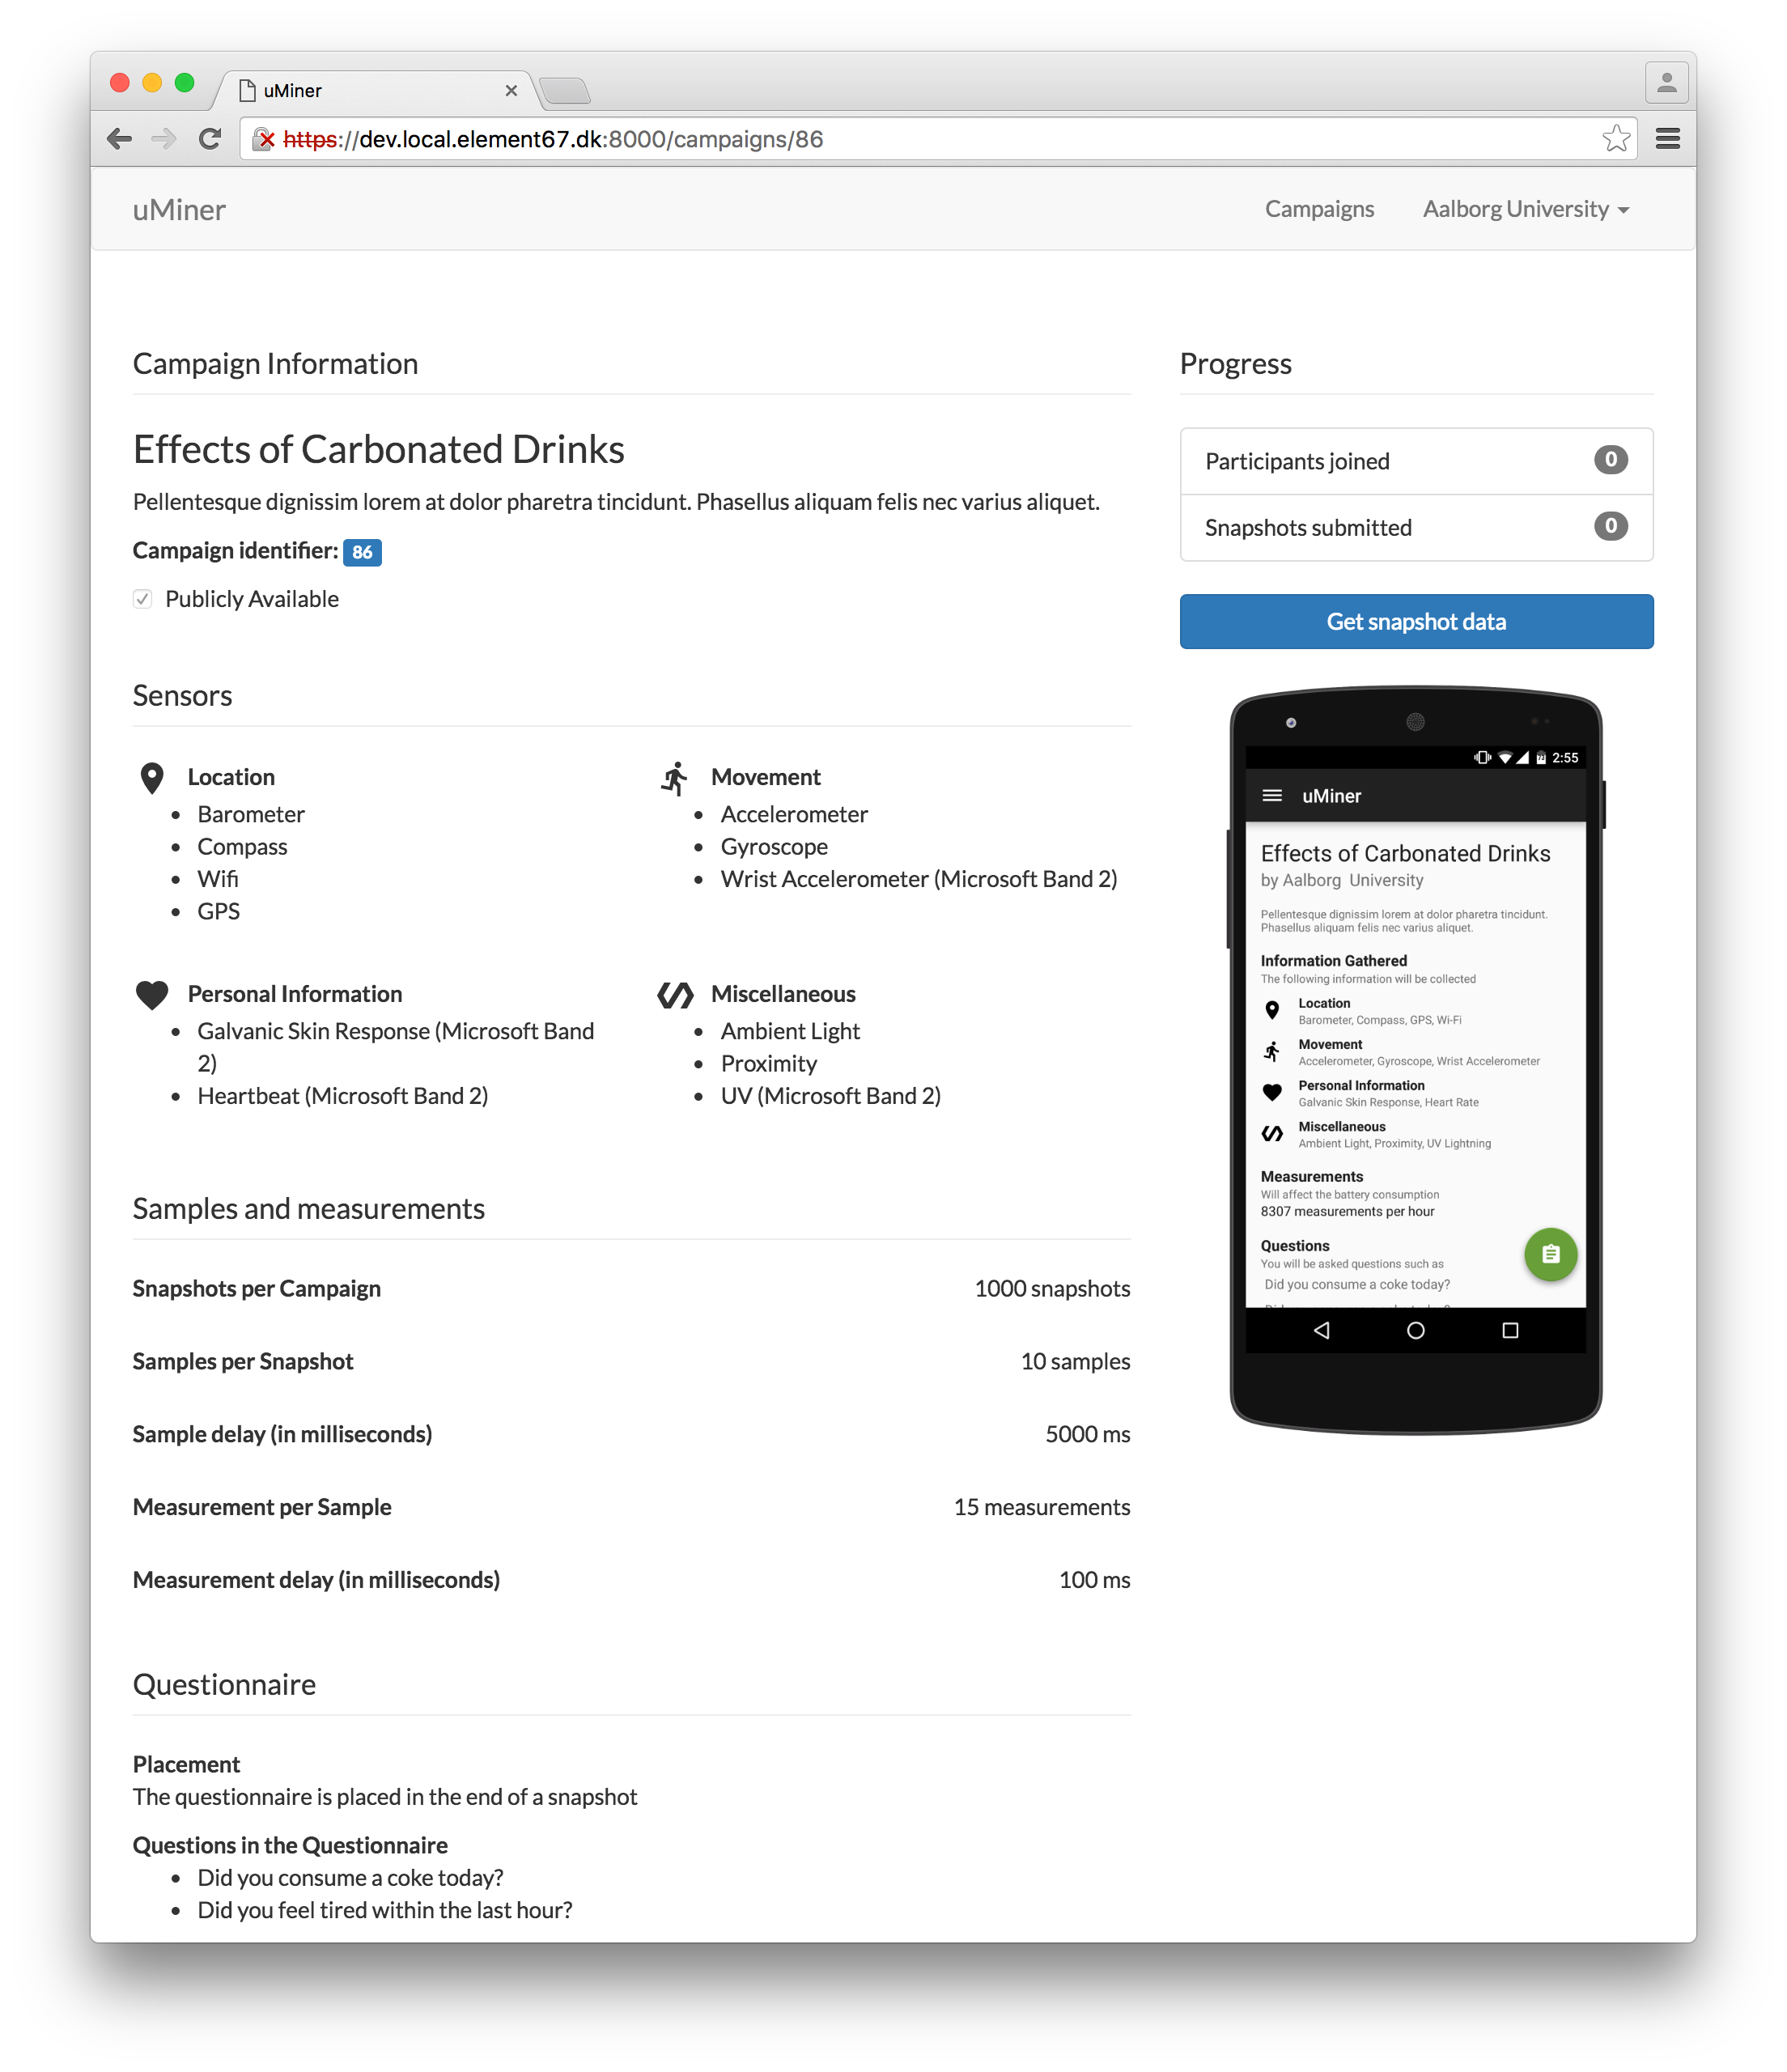
\includegraphics[width=\linewidth]{user_interfaces/web/web_view_campaign}
\caption{Viewing Campaigns.}
\label{fig:web_view_campaign}
\end{figure}
\FloatBarrier

\subsection{Editing and Deleting Campaigns}

\todo[inline]{Skriv at vi har valgt at gøre det umuligt at redigere og slette campaigns. Slet gad vi ikke. Edit krævede for meget arbejde da ændringerne skulle reflekteres ned på alle devices der var tilmeldte, som skulle opdatere deres timings, og slette alt det data de havde indsamlet. Long story kort: Det ville være NÆSTEN det samme som at slette og genoprette campaignen hvis edit funktionalitet skulle blive implementeret.}